\chapter{Accessivity tools and demonstrations}

With the entire system designed and programmed on the FPGA, it's time to test it. But before that, 
one needs tools to allow to write in the memories of the machine from Linux, on the ARM processor. 
In addition to that, tools simplifying the development on the system are presented. After the 
presentation of the different tools, the different assembler demonstrations are detailed.

\section{Tools}

\subsection{Beta assembler}

The first tool is a tool that was developed by Romain Mormont. It allows the assembly of assembly 
code using the ISA described earlier in the report into machine code for beta machine. This tool 
had already been created before this work, so it was decided to take advantage of it and not 
reinvent the wheel. Some minor modifications were made to add a binary file backup that could be 
used for programming the beta machine of this work, to add the exit instruction and to remove the 
div instruction.

\subsection{Beta utils}

Beta utils is a utility that allows access to memory and system control from the ARM processor. In 
fact, to do this it is enough to write and read in the space address of the bridge avalon on which
a slave is connected in QSys. To have access to a given slave, it is necessary to add its offset 
(specified in QSys) to the starting address of the bridge in the physical memory. The start and end 
addresses of each bridge are constant and specified in Figure \ref{fig:cyc5/address_space}. 

To keep things simple, it was decided to implement everything in the user space of the OS. Beta 
utils is therefore only an application. This application does not have direct access to the 
physical addresses. In order for it to be able to read and write to specific locations in physical 
memory, a mapping must first be created between the physical memory and the virtual memory of the 
Beta utils process. To do this, the system call mmap is used. This creates a mapping and returns a 
pointer allowing access to the specified physical memory in a contiguous manner from the virtual 
memory. This means that $pointer + n$ corresponds to the nth element of the mapped physical region. 
This solution is not the fastest but is more than sufficient for the operations performed by Beta 
utils and has the merit of being simple. 

For the communication with the memories, the tool allows two operations. Both can only be done 
when the system on FPGA is stable, in other words when the alive signal is low. The first one is 
writing. This one allows to write the content of a binary file in the chosen memory, with a certain 
offset in it. The use of this operation is described in Figure \ref{fig:tools/program}.

\begin{figure}[H]
    \centering
    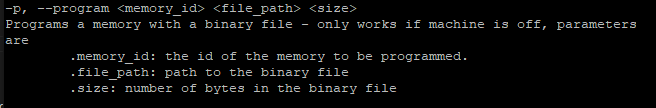
\includegraphics[scale=1]{Chapter7-Tools-Demos/res/utils_program.PNG}
    \caption{Program command}
    \label{fig:tools/program}
\end{figure}

Reading is done from a starting 
offset to an ending offset. The bytes are simply displayed, there is no saving to a file. 
Figure \ref{fig:tools/read} shows its use. The memory identifiers are IM for 
instruction memory, DM for data memory, RF for register file, IO for io memory and MK for mask 
memory.

\begin{figure}[H]
    \centering
    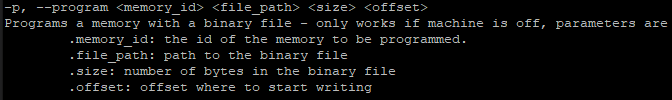
\includegraphics[scale=1]{Chapter7-Tools-Demos/res/utils_read.PNG}
    \caption{Read command}
    \label{fig:tools/read}
\end{figure}

To switch on and off the system, two operations are provided, they are given in 
Figure \ref{fig:tools/st_sd}.

\begin{figure}[H]
    \centering
    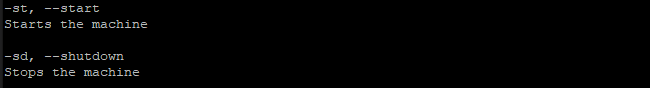
\includegraphics[scale=1]{Chapter7-Tools-Demos/res/utils_power.PNG}
    \caption{Start and shutdown commands.}
    \label{fig:tools/st_sd}
\end{figure}

\subsection{Mask Drawer}

The mask drawer is a small tool coded in python developed for this work. It provides a graphical 
interface, shown in Figure \ref{fig:tools/mask_drawer}, that allows editing of masks. In the window 
there are five buttons. 
Four are used to select the state to be applied: keep, primary color, secondary color and clear. 
Once a state has been selected, simply click on the grid to change the state of the pixel. A square 
on the grid represents a pixel. If the mouse is held down on the left button, all the cells through 
which the cursor passes will have their state changed. It is also possible to simply click one cell 
by one cell. The right click is a shortcut to the keep state. Once the mask is drawn, it can be 
saved as a binary file by clicking on generate. Note that the mask drawer takes as argument the 
name of the file, without its extension. If this file already exists, it is opened and its edition 
can be resumed. If it does not exist, it is created. 

\begin{figure}[H]
    \centering
    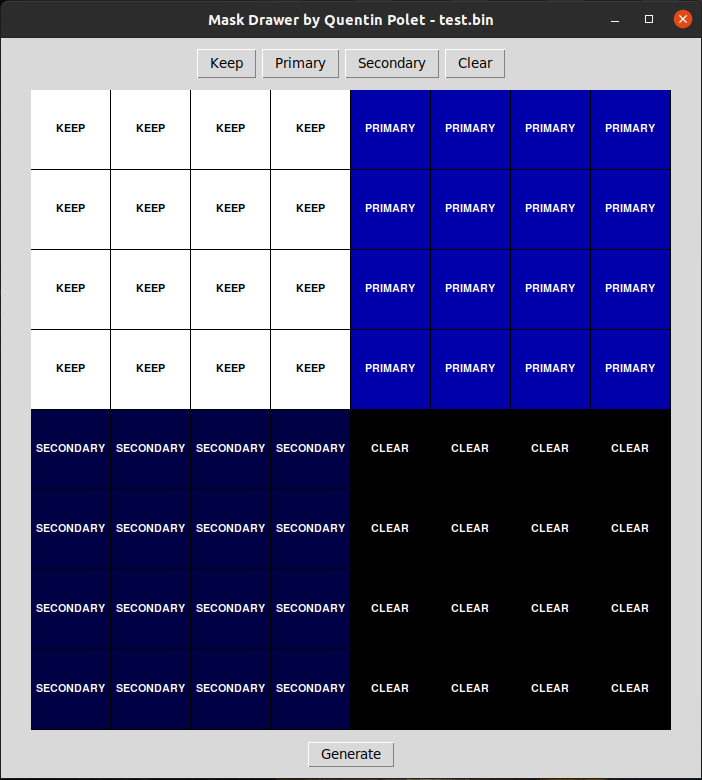
\includegraphics[scale=0.5]{Chapter7-Tools-Demos/res/mask_drawer.png}
    \caption{Mask drawer}
    \label{fig:tools/mask_drawer}
\end{figure}

\section{Assembler desmonstrations}

Once the implementation of the system was completed, I was fortunate to be put in contact and have 
a discussion with two Intel employees, Nadel Alexander research scientist at Intel Israel and 
Gyuszi Suto principal engineer at Intel Oregon. During this discussion, these two people provided 
guidance on how it was appropriate to verify the system. The easiest way, for them, was to perform 
several demonstrations using the different parts of the system and verify experimentally that 
everything worked. This is far from the verification methods presented in an article 
explaining how verification is done at Intel that Nadel Alexander suggested reading. But doing such 
verification (formal verification and so on) would be the work of one or more master theses. 
Therefore, after discussion and reading of the article, it was decided to use the experimental 
approach, in addition to the simulations done on the ALU to prove that some confidence can be given 
to this system. The demonstrations are explained in this section.

\subsection{Assembler libraries}

Before moving on to the demos, this section briefly describes the libraries written for this job to 
simplify programming for users. The first one gpu\_utils provides all the functions to use the gpu. 
io\_utils provides exactly the same thing but to access the IOs of the IOU. And finally, there is 
the stack library which provides an implementation of stack. The different functions of these 
libraries are all documented in their files.

\subsection{Hanoï towers}

The first demonstration is to solve the Towers of Hanoi problem graphically. The Hanoi Towers 
problem consists of moving a stack of N elements of different dimensions that are ordered from the 
widest at the base to the narrowest at the top of the tower. To do this, the elements can be moved 
one by one and placed on a stack. There are three stacks. The tower is initially placed on one of 
them. For a move to be valid, the element at the top of the stack on which the moved element is to 
be placed must be larger than this one. In other words, an element must always be placed on top of 
a larger element. The goal is then to move the whole tower to another stack. When the demo is 
launched on the machine, a tower of height 6 is created on the first of the three piles and then 
the program solves the problem step by step, until the tower is placed in the center. Between each 
movement, there is a wait so that the resolution is possible to follow. This demonstration in 
action on the system developed in this work is available on 
\href{https://www.youtube.com/watch?v=0W0SXzncl-Q}{YouTube}.

\subsection{Stacker game}

Solving the Towers of Hanoi does not include the IOs part, so a small game with interractions has 
been added. However, here the task was delegated to a friend, 
Gauderic Schnackers who is a graduated physicist engineer. This allowed two things. Firstly to 
validate the whole system but also to validate the accessibility of the system. This is important 
as the system is to be used as laboratory material in an introductory course. Since Gauderic had 
never worked so low on a machine and never programmed in assembler, he was the perfect tester. 

This game is very simple, the goal is to stack sticks of a certain length to the top of the screen. 
If two sticks don't stack perfectly, the protruding part of the stick is subtracted and the next 
stick to be placed is shorter. If the stick is completely consumed before reaching the top, the 
player loses the game. Again, this demonstration performed on the system of this work is available 
on \href{https://www.youtube.com/watch?v=yHJDM_ckR1g}{YouTube}.